
\subsection{Алгоритмы для вычисления параметров волн}


Раздел~\ref{sec:wave_theory} был целиком посвящен методике определения параметров подходящих к берегу волн и вычислению передаваемой на него энергии.
В следующем за ним разделе~\ref{sec:wer_calculation}, в свою очередь, формулировались гипотетические индексы, способные служить основой к качественной оценке устойчивости береговой линии.
Сразу отметим, что идеи, формулы и подходы описанные в приведенных разделах в полном объеме использованы в реализованной программе.

Тем не менее, обратив внимание на большой объем требуемых к выполнению операций становятся очевидной большая ресурсоемкость требуемых вычислений. 
Отчего буквальное выполнение всех вычислений \enquote{в лоб} приведет, очевидно, к высокой алгоритмической сложности исполняемой программы.

Принимая во внимание то, что использованные в работе пакеты для работы с геопространственными данными используют внутри себя высокопроизводительные алгоритмы наиболее перспективным способом к ускорению выполнения вычислений является простой и проверенный способ -- просто не считать лишнего.
Из чего цель следующих разделов лишь \enquote{подсветить} принятые в программе допущения и алгоритмические решения.

\subsubsection{Вычисление предельно-значимой длины разгона}

Одной из фундаментальных величин необходимой для вычисления параметров разгона волн на открытой, глубокой, воде является определение длины разгона ветра над открытой водой, определяемое трассировкой лучей от рассматриваемой точке в направлениях обратном направлению ветра.
Фактически эта работа сводится к вычислению длины геодезической прямой (по геоиду) от точки расчета до первой точки на суше вдоль требуемого вектора.

Алгоритмы трассировки лучей активно используются в компьютерной графике, но в нашей задаче такая точка встречи может оказаться как в нескольких десятках метров на закрывающем берег пирсе, такми и в тысячах километров на противоположном берегу океана.
Такая постановка задачи не может не привести к трудностям с загрузкой глобальных береговых данных и работе с ними.

Любознательность заставила проверить границы дозволенных вычислений в рамках глобальных моделей.
Так вычисления, включающие всю акваторию Черного моря, еще с трудом выполнимы, но попытка трассировки через весь Тихий океан, ожидаемо, завершилась безрезультатно.

При анализе формул в разделе~\ref{sec:deep_whater_wave} упоминалось, что формулы~\eqref{eq:smb_hs} и~\eqref{eq:smb_tp} включающие в себя функции гиперболического тангенса при определенном балансе отношения скорости ветра и длины разгона ветра переходят в насыщенное состояние~\eqref{eq:smb_hs_approx} и~\eqref{eq:smb_tp_approx}.

Границей перехода в насыщенное состояние можно принять равенство входящего в формулы $\tanh(\cdot)=\alpha$, где $\alpha$ -- это коэффициент, определяющий накопленную от максимально возможной высоту волны, возможную при скорости ветра $U$.
Ограничивая $\alpha$ величинами 0.9, 0.95 или 0.99 мы можем найти границу после которой длина разгона уже будет в меньшей степени влиять на параметры волн.
При этом разница $k$ между $1 - \alpha$ может быть учтена путем умножения полученных значений $T_p$, $H_s$ на соответствующую величину $k$.

Посмотрим еще раз на полную формулу вычисления средней высоты волны~\eqref{eq:smb_hs}:
\begin{equation}
    H_s = 0.283\,\frac{U^2}{g}\, \tanh\!\bigl(0.53\,X^{0.75}\bigr)
\end{equation}
и приравняем гиперболический тангенс коэффициенту $\alpha$ выразив множитель $X$:
\begin{equation}
    \tanh\!\bigl(0.53\,X^{0.75}\bigr)=\alpha
    \;\Rightarrow\;
    0.53\,X^{0.75} = \operatorname{artanh}(\alpha)
    \;\Rightarrow\;
    X = \left[\frac{\operatorname{artanh}(\alpha)}{0.53}\right]^{\frac{1}{0.75}}.
\end{equation}

Численные значения коэффициента $X$ при этом легко вычислить, после чего из определения $X = gF/U^2$:
\begin{equation}
    F_{\max,\alpha}(U) = \frac{U^2}{g}\,X_\alpha.
\end{equation}

Для названных порогов $\alpha$ результаты приведены в таблице~\ref{tab:hs_levels_FHmax}.

Аналогично для периода волны $T_p$ введем коэффициент $\beta$.
Пиковый период волны $T_p$, соответствующий максимуму спектра энергии, выражается через $X$ как:
\begin{equation}
    T_p = 7.54\,\frac{U}{g}\, \tanh\!\bigl(0.833\,X^{0.375}\bigr).
\end{equation}

Введем аналогично критерий «почти полностью развитого» периода:
\begin{equation}
    \tanh\!\bigl(0.833\,X^{0.375}\bigr) = \beta,
\end{equation}
где $\beta = 0.9,\;0.95,\;0.99$.

Отсюда:
\begin{equation}
    0.833\,X^{0.375} = \operatorname{artanh}(\beta)
    \;\Rightarrow\;
    X^{0.375} = \frac{\operatorname{artanh}(\beta)}{0.833}
    \;\Rightarrow\;
    X_\beta = \left[\frac{\operatorname{artanh}(\beta)}{0.833}\right]^{\frac{1}{0.375}}.
\end{equation}
Дальше, как и для высоты, используем $X = gF/U^2$:
\begin{equation}
    F_{\max,\beta}(U) = \frac{U^2}{g}\,X_\beta.
\end{equation}

Соответствующее приближение периода в результате будет:
\begin{equation}
    T_{p,\beta}(U) = 7.54\,\frac{U}{g}\,\beta.
\end{equation}

Это приближене обосновано тем, что при выбранном пороге гиперболический тангенс уже равен $\beta$, и период составляет долю от предельного $T_{p,\mathrm{FDS}} = 7.54\,U/g$.

Сводная таблица вычисленных коэффициентов представлена в таблице~\ref{tab:tp_levels_FTmax}.

\begin{landscape}
    \begin{table}
        \caption{-- Значения функции $F_{H,\max}(U)$ для различных уровней по $H_s$}
        \label{tab:hs_levels_FHmax}
        \centering
        \begin{tabular}{l c c l}
            \toprule
            \textbf{Уровень по $H_s$} &
            \boldmath$\alpha$\unboldmath &
            \boldmath$X_H(\alpha)$\unboldmath &
            \textbf{Формула $F_{H,\max}(U)$} \\
            \midrule

            $90\%$ от $H_{s,\mathrm{FDS}}$ &
            $0{.}90$ &
            $\approx 3{.}90$ &
            $F_{H,\max,90}(U) \approx 3{.}90\,\dfrac{U^2}{g}$ \\

            $95\%$ от $H_{s,\mathrm{FDS}}$ &
            $0{.}95$ &
            $\approx 5{.}23$ &
            $F_{H,\max,95}(U) \approx 5{.}23\,\dfrac{U^2}{g}$ \\

            $99\%$ от $H_{s,\mathrm{FDS}}$ &
            $0{.}99$ &
            $\approx 8{.}54$ &
            $F_{H,\max,99}(U) \approx 8{.}54\,\dfrac{U^2}{g}$ \\

            \bottomrule
        \end{tabular}
    \end{table}

    \begin{table}
        \caption{-- Значения функции $F_{T,\max}(U)$ и периода $T_p(U)$ для различных уровней по $T_p$}
        \label{tab:tp_levels_FTmax}
        \centering
        \begin{tabular}{l c c l l}
            \toprule
            \textbf{Уровень по $T_p$} &
            \boldmath$\beta$\unboldmath &
            \boldmath$X_T(\beta)$\unboldmath &
            \textbf{Формула $F_{T,\max}(U)$} &
            \textbf{Формула $T_p(U)$} \\
            \midrule
            $90\%$ от $T_{p,\mathrm{FDS}}$ &
            $0{.}90$ &
            $\approx 7{.}4$ &
            $F_{T,\max,90}(U) \approx 7{.}4\,\dfrac{U^2}{g}$ &
            $T_{p,90}(U) = 0{.}90 \cdot 7{.}54\,\dfrac{U}{g}$ \\
            $95\%$ от $T_{p,\mathrm{FDS}}$ &
            $0{.}95$ &
            $\approx 12{.}9$ &
            $F_{T,\max,95}(U) \approx 12{.}9\,\dfrac{U^2}{g}$ &
            $T_{p,95}(U) = 0{.}95 \cdot 7{.}54\,\dfrac{U}{g}$ \\
            $99\%$ от $T_{p,\mathrm{FDS}}$ &
            $0{.}99$ &
            $\approx 30{.}7$ &
            $F_{T,\max,99}(U) \approx 30{.}7\,\dfrac{U^2}{g}$ &
            $T_{p,99}(U) = 0{.}99 \cdot 7{.}54\,\dfrac{U}{g}$ \\
            \bottomrule
        \end{tabular}
    \end{table}
\end{landscape}

Как видно из таблицы~\ref{tab:tp_levels_FTmax}, $X_T$ здесь значительно больше, чем соответствующие коэффициенты  $X_H$ для высоты, что отражает более медленное «дорастание» периода до предела по сравнению с высотой при ограничении длины разгона.
Таким образом, для практического выбора $F_{\max}$ по целесообразнее использовать эти множители.

Зависимость между этими показателями от скорости ветра представлена графиками на рисунке~\ref{pic:Tp_Hs_Fetch_limiths}.

\begin{figure}
    \begin{center}
	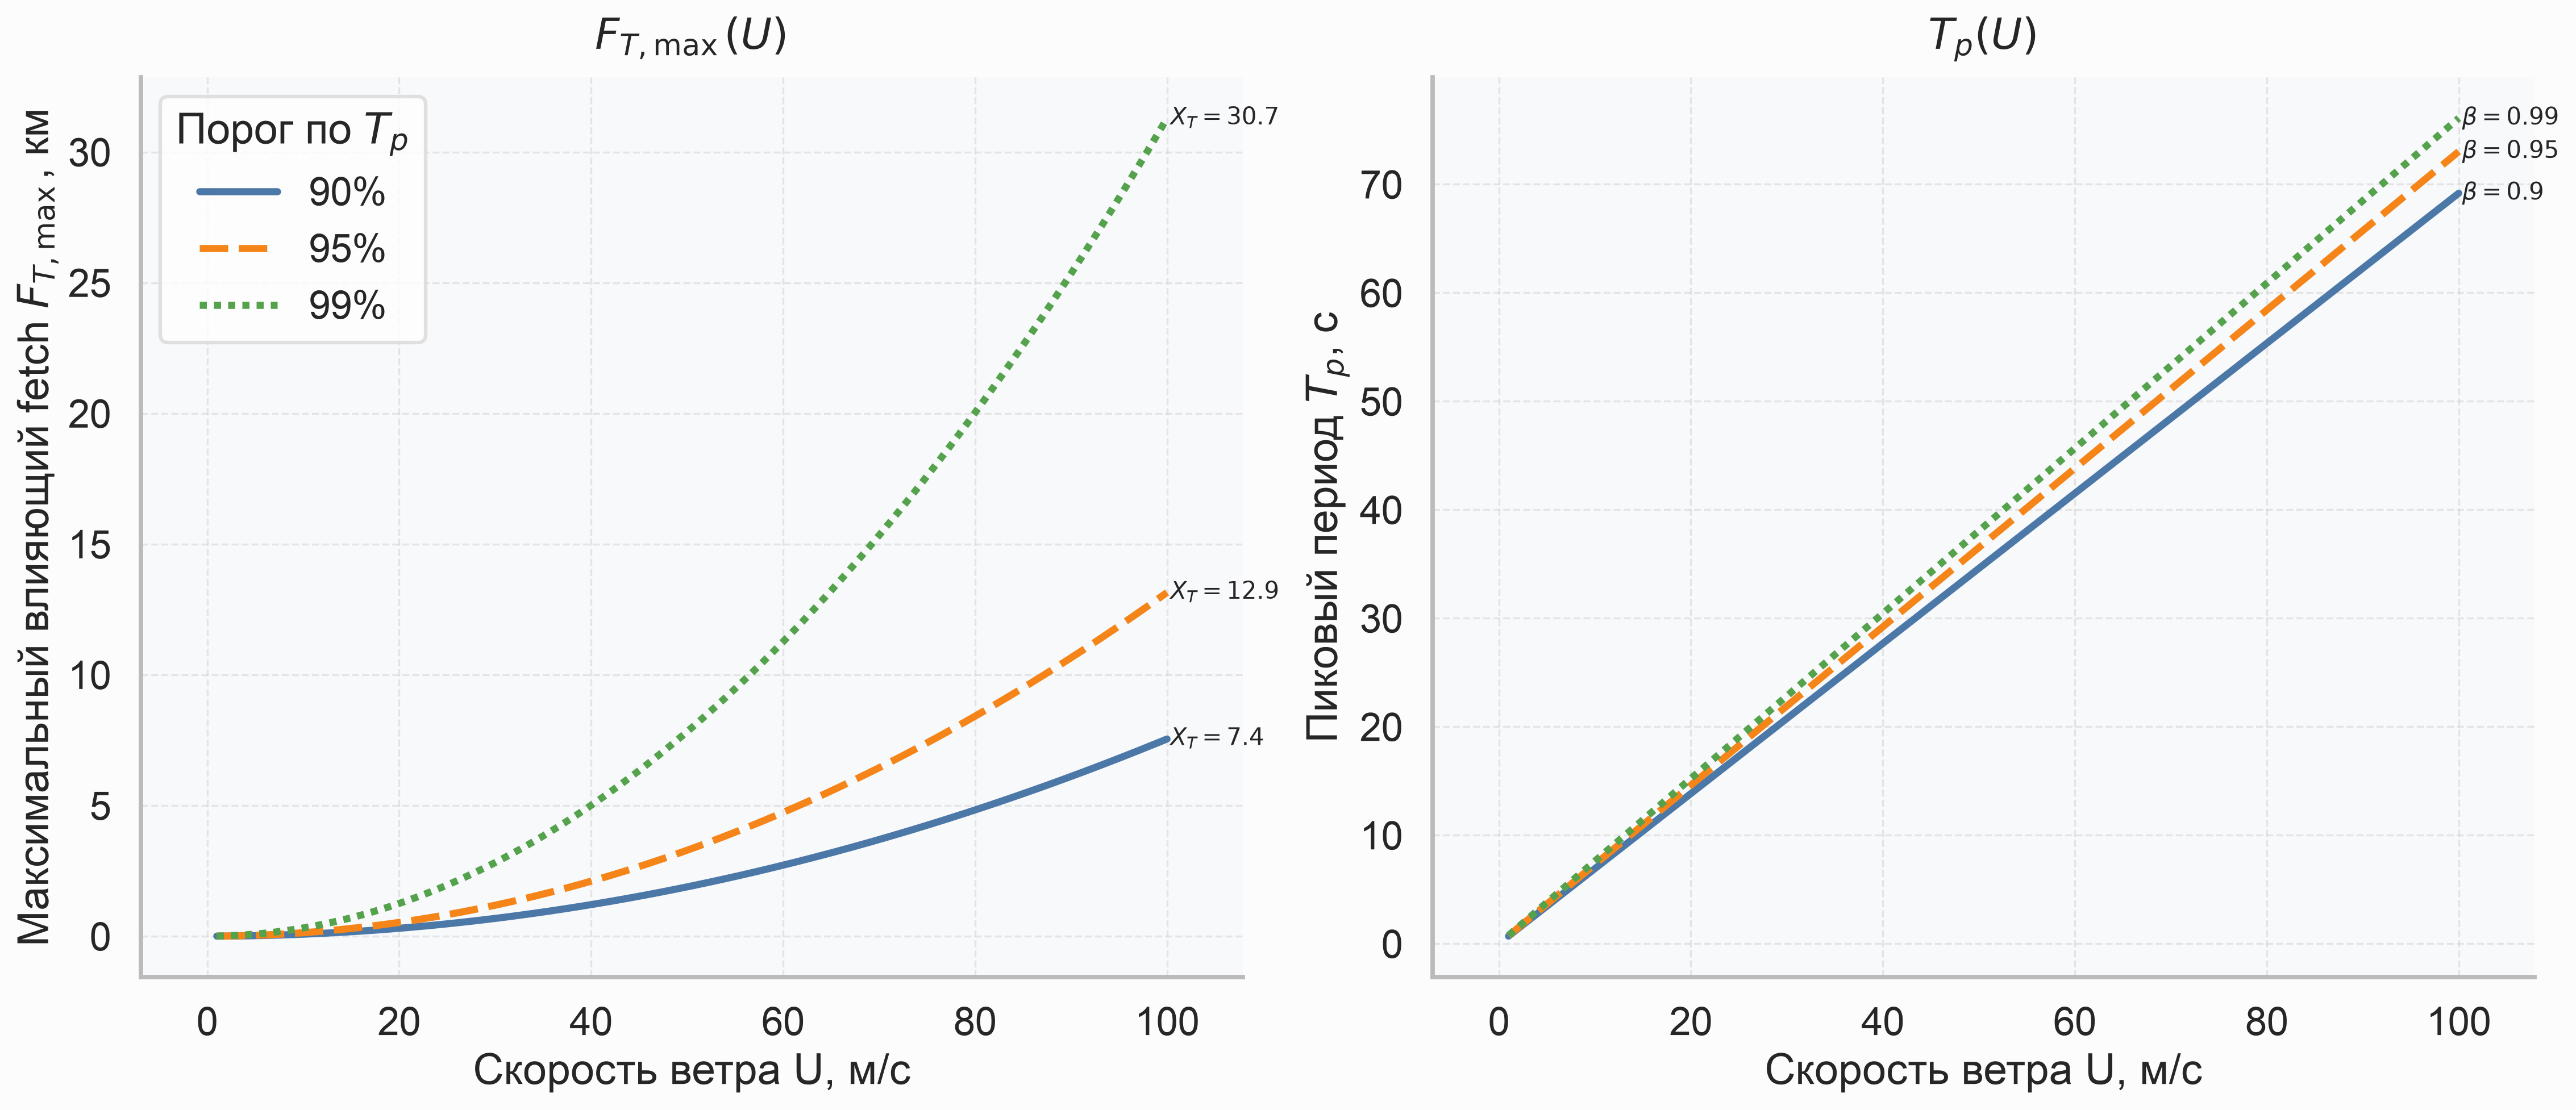
\includegraphics[width=\textwidth]{fig/part_2/Tp_Hs_Fetch_limiths.png}
	\caption{-- Зависимости предельных величин разгона и пикового периода волны от скорости ветра}
	\label{pic:Tp_Hs_Fetch_limiths}
    \end{center}
\end{figure}


\subsubsection{Подготовка береговой линии для вычисления длины разгона}

В предыдущем разделе были получены значения максимально влияющих длин разгона ветра.
Практически это значение следует рассматривать как величину пространственного буфера, внутри которого следует искать точку пересечения трассирующего луча с противоположным берегом.
Не превышение заданного порога определит неполную \enquote{силу} волны и, как следствие, ее меньшее разрушающее воздействие.

Технически, имея статистику скорости ветров за рассматриваемый период, размер этого буфера может быть вычислен строго для каждой точки по отдельности либо для максимального значения скорости ветра по всей совокупности.
Однако эмпирический опыт показал, что для относительно локальных расчетов увеличение зоны расчета даже на 100 км не приводит к существенным вычислительным задержкам.

В любом случае необходимость вычисления длин разгона ветра не может быть выполнена в пределах заданной на первом этапе береговой линии и требует своего расширения.
В разработанной программе это реализовано как передача в расчет дополнительного фрагмента береговой линии, покрывающей необходимый дополнительный буфер.
В перспективе эта операция будет упрощена путем автоматического \enquote{вырезания} из набора данных S2Coast-2023 участка, определенного как сумма ограничивающей геометрии исходных данных с шириной буфера.

Однако разная точность и содержание используемых данных не позволит использовать его в вычислениях сразу, так как несовпадение береговых линий в локальной окрестности береговых точек приведет к появлению многочисленных коллизий при трассировке.
Исходя их этого, векторные данные для вычисления длин трасс разгона в программе формируются как комбинация расширенного и исходного слоя береговых линий.

Для этого из расширенного, внешнего, слоя автоматически вырезаются объекты, попавшие внутрь исходной ограничивающей геометрии (бибокса), а линии пересекаемые им обрезаются по его границам.
После этого исходные данные помещаются взамен удаленных.
При этом, в случае использования различных источников данных, на границах исходного бибокса возникнут топологические разрывы линий.
Хотя шанс попадания трассирующего луча в подобный разрыв можно принять как статистически маловероятный в программе эти разрывы заполняются поиском ближайшего соседа вдоль границы бибокса обрезки.

После этого полученный слой используется в качестве опорного для вычисления трассировки.

\subsubsection{Алгоритм трассировки для вычисление длины разгона ветра}

Описанные ранее подходы служат всего лишь прелюдией к одному из наиболее ресурсоемких этапов выполнения метода -- вычислению длин разгона ветра путем трассировки.

Накопленные данные о направлениях ветра определены непрерывно в интервале от $0^\circ$ до $360^\circ$ градусов.
Очевидно, что качество расчета будет напрямую зависеть от степени дискретизации интервалов рассматриваемых направлений, которые, в свою очередь, должны быть обеспечены объемом используемой выборки.
Так как используемые данные хранят в себе историю более чем 85 лет наблюдений в работе был выполнен расчет по 360 направлениям для каждой точки.
В перспективе этот параметр должен подлежать анализу и, вероятнее всего, сокращению, так как он физически определяет дальнейшее время расчетов, но пока посчитаем по максимуму.

Технически сами алгоритмы трассировки уже включены в библиотеку \texttt{shapely}, однако просто ничего никогда не получается -- этот случай исключением не стал.

Во-первых, что мы имеем?
У нас есть набор точек на береговой линии и мы зачем-то считали для них вектора нормали...
Время этих векторов пришло!

Что произойдет если выполнить трассировку сразу для точки лежащей на береговой линии?
Лучи пойдут во все стороны, как в сторону моря (что нам и нужно), так и в сторону суши (что для нас не приемлемо).
Если проигнорировать это, то в результате мы сформируем ситуацию аналогичную случаю, когда бесконечно узкая линия суши омывается с двух сторон морем.

Математически избежать этого не сложно.
Если вектор нормали направлен в сторону моря (это является необходимым условием заявленным в разделе~\ref{sec:task_intro}) мы можем временно сместить точку вдоль этого направления на небольшое расстояние.

Для этого из нормали строится вектор смещения длиной (\texttt{offset\_m}):
\begin{equation}
    (dx, dy) = \text{offset\_m} \cdot 
    \begin{cases}
    \sin(\text{normal}),\\
    \cos(\text{normal}).
    \end{cases}
\end{equation}

А координаты стартовой для лучей точки вычисляются как:
\begin{equation}
    (x_0, y_0) = (x_s + dx,\, y_s + dy).
\end{equation}

После этого точка окажется со всех сторон окружена морем и мы можем честно посчитать длины трасс во всех требуемых направлениях.

Но по всем ли направлениям мы можем посчитать их верно и по всем ли они нам нужны?
Ответы на эти вопросы: нет и нет.
Не до конца понятно почему, но библиотека \texttt{shapely} не всегда может определить верную точку пересечения с отрезками, лежащими очень близко к точке, вследствие чего луч \enquote{пробивается} сквозь берег, что нарушает верность расчета.
Стабильно решить эту проблему без понижения качества результатов не удалось, но это оказалось к лучшему.

Если мы уверены, что точка лежит на берегу, а вектор нормали направлен в море, то зачем нам считать в обратную ему направление?
Незачем!
В результате честная трассировка по всем направлениям становится не нужна.

В результате перед трассировкой каждое направление проверяется, не находится ли оно \enquote{в сухопутном секторе}. 
Для чего рассчитывается разность:
\begin{equation}
    \Delta = (\text{azimuth} - \text{normal}) \bmod 360.
\end{equation}

Если $90^\circ \le \Delta < 270^\circ$, направление считается обращенным в сторону суши (внутрь берега).
Для таких направлений трассировка не выполняется, а длина разгона считается равной величине принятого смещения \texttt{offset\_m}.
Дополнительно эти направления помечаются специальным флагом, позволяющим пропустить их при вычислении последующих расчетов.

Для оставшихся \enquote{морских} направлений трассировка считается честно.
По пространственному индексу выбирается подмножество береговых сегментов, которые пересекают MBR (Minimum Bounding Rectangle) луча.
Внутри полученного набора сегментов вычисляются точки пересечения линий с лучем.
После чего считаются расстояния от стартовой точки и выбирается точка с минимальной дистанцией. 

В случае, если луч не пересек ни одного сегмента береговой линии -- это значит он направлен в сторону открытого моря.
Величина разгона вдоль этого направления в расчете принимается равной участвующей при определении буфера эффективной длине прогона луча $F_{T,\max}$.

Результаты трассировки представлены на рисунке~\ref{pic:Трассировка_лучей}. На фрагменте \enquote{А} показаны расчеты по 360 азимутальным направлениям для каждой точки, на фрагментах \enquote{Б} - \enquote{Г} -- для 10 напвлений в разных масштабах района Цемесской бухты.

\begin{figure}
    \begin{center}
	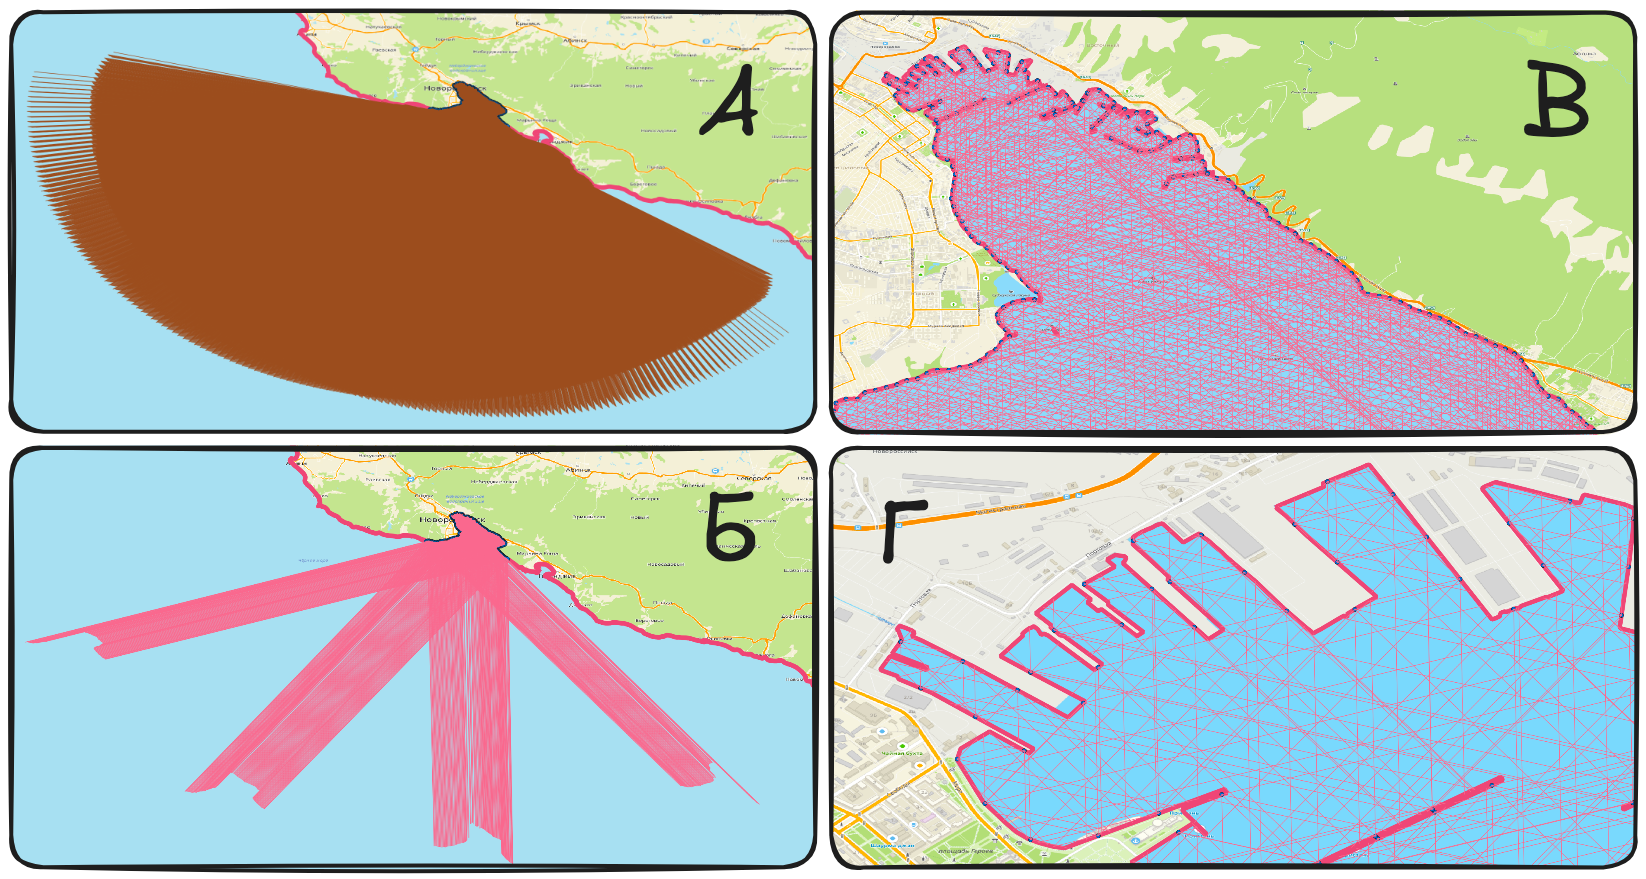
\includegraphics[width=\textwidth]{fig/part_2/alghoritm/Трассировка_лучей.png}
	\caption{-- Пример результатов выполнеия трассировки лучей для расчета длины разгона ветра}
	\label{pic:Трассировка_лучей}
    \end{center}
\end{figure}